
% Copyright (c) 2015 - 2019 Mario Mlačak, mmlacak@gmail.com
% Published as Public Domain work, under CC0 1.0 Universal Public Domain Dedication. See LICENSING, COPYING files for details.

% Classical Chess -----------------------------------------------------
\chapter*{Classical Chess}
\addcontentsline{toc}{chapter}{Classical Chess}
\label{ch:Classical Chess}

\begin{flushright}
\parbox{0.8\textwidth}{
\emph{A great war leaves the country with three armies -
an army of cripples, an army of mourners, and an army of thieves. \newline
\hspace*{\fill}{\textperiodcentered \textperiodcentered \textperiodcentered \hspace*{0.2em} German proverb} } }
\end{flushright}

\noindent
About classical chess is written really everything already, and I
have nothing to add, except for introduction on how to read the book.

\clearpage % ..........................................................

\TODO :: introduction \newline
\textrightarrow arrows \& colors \newline
\textrightarrow markers, texts (enumerations vs. labels) \newline
\textrightarrow steps, step-fields, capture-fields \newline
\textrightarrow rush \newline
\textrightarrow context, exceptions \newline
\textrightarrow chessboard sides, navigation \newline
\textrightarrow basic terminology: turn, move, cycle, figure, ... \newline

\clearpage % ..........................................................

\noindent
\begin{figure}[t]
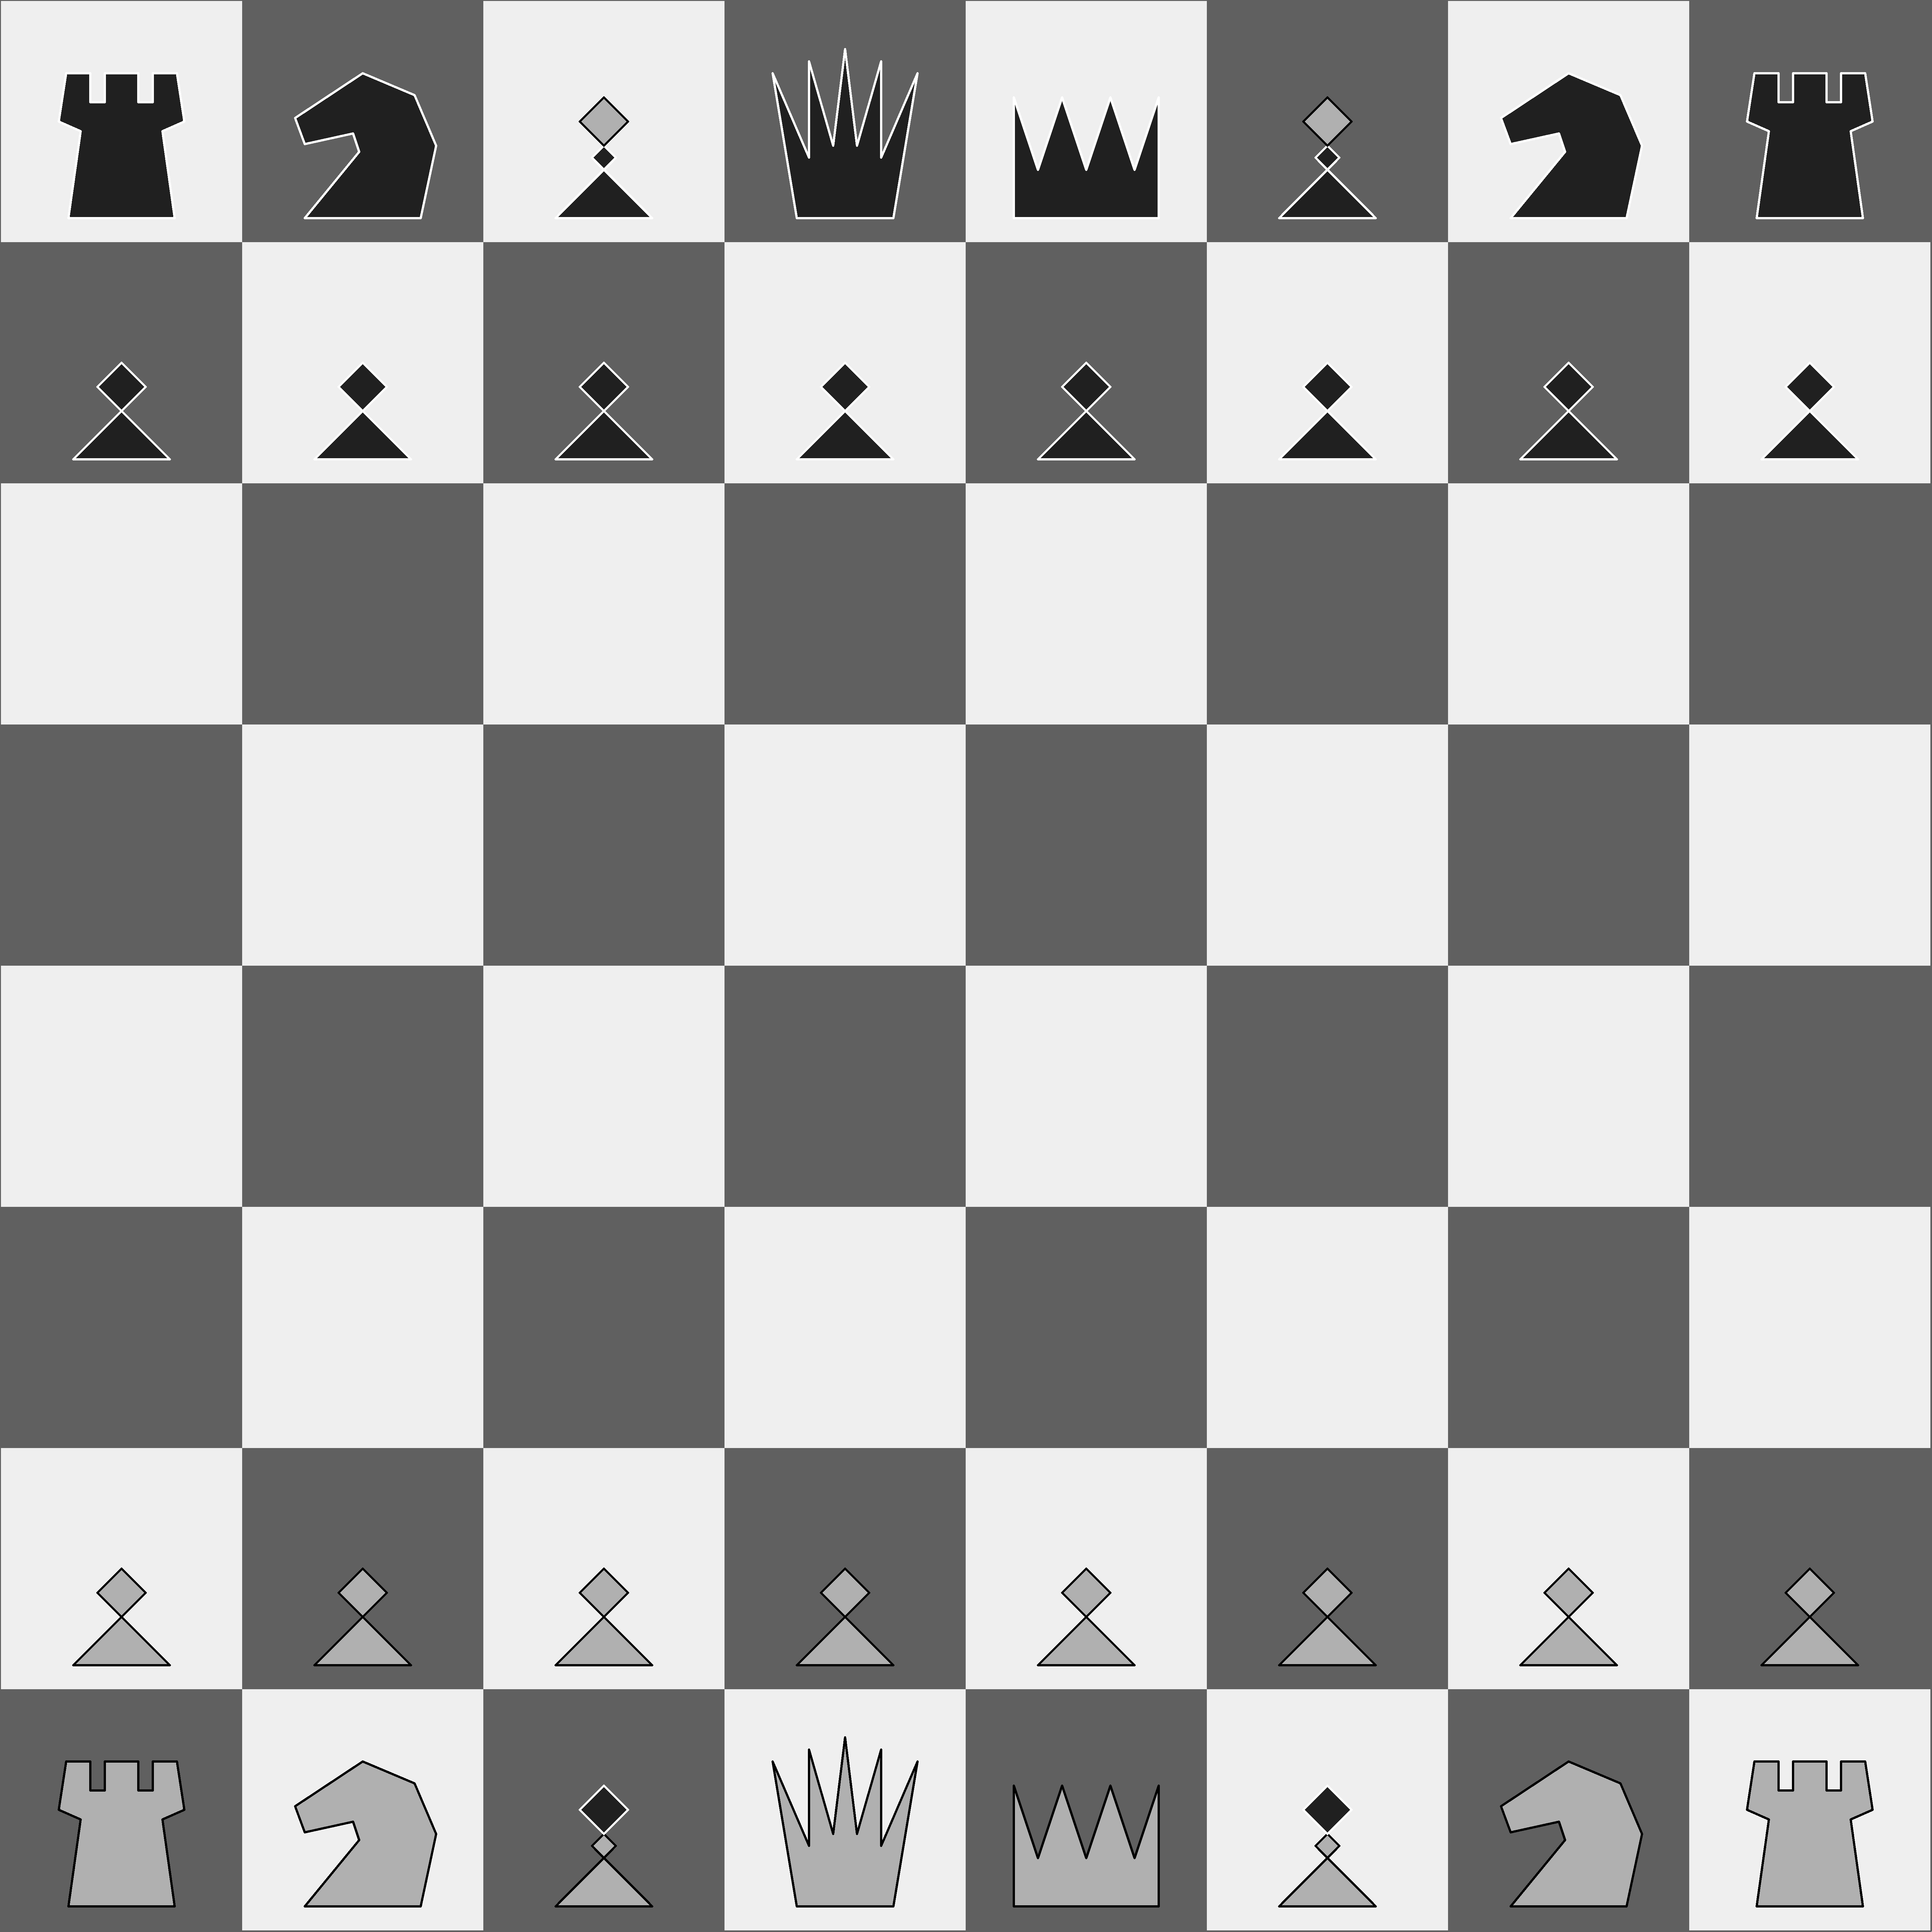
\includegraphics[width=1.0\textwidth, keepaspectratio=true]{boards/02_classical.png}
\caption{Classical board}
\label{fig:02_classical}
\end{figure}

\clearpage % ..........................................................
% ----------------------------------------------------- Classical Chess
